\documentclass[document.tex]{subfiles}
\begin{document}

\chapter{Metody równoległego przetwarzania danych}

\section{Współbieżność w ramach architektury CPU}
\indent Rozwój technologii wytwarzania układów elektronicznych, doprowadził do 
rozpowszechnienia mikroprocesorów, które zawierają wszystkie komponenty w jednym
układzie scalonym. Ponadto pojedynczy układ zawiera obecnie więcej niż jeden procesor - rdzeń, każdy z nich posiada 2
wątki sprzętowe. Powoduje to coraz większą popularność wykorzystywania współbieżnego modelu programowania współczesnych wielordzeniowych procesorów.\cite{OS_Stallings}
\cite{Computer_Architecture_Patterson_Hennesy}
\\
\indent Każdy procesor składa się z :
\begin{itemize}
\item jednostki artmetyczno logicznej - ALU(arithmetic logical unit).
\item zestawu rejestrów
\item jednostki kontrolnej - CU(control unit)
\end{itemize}

%wrucic tu rysunek - schemat blokowy procesora
\begin{figure}[h]
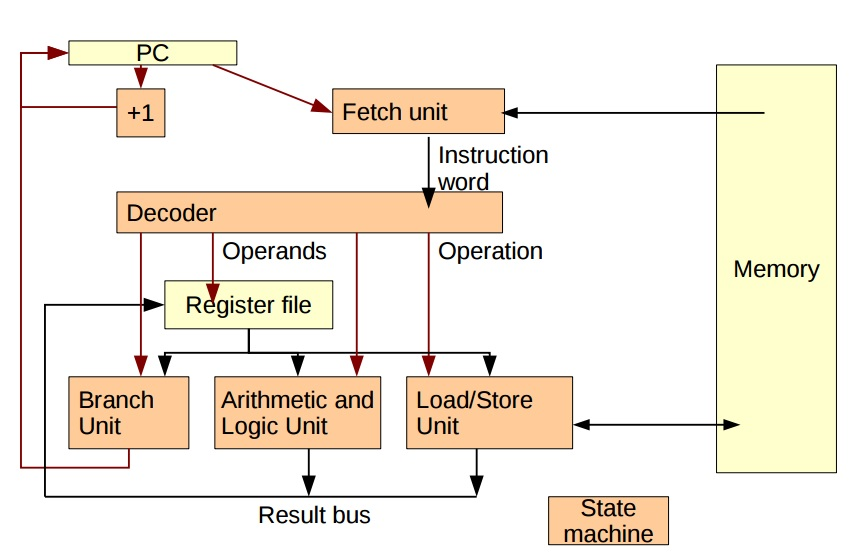
\includegraphics[scale=0.5]{cpu_scheme}
\caption{Schemat cyklu pobierania i wykonania instrukcji przez CPU \protect\cite{OS_Stallings}}
\label{fig:cpu_scheme}
\end{figure}

%opis cuklu ehzekucji programu
Jednostka arytmetyczno logiczna(\textbf{ALU})
jest odpowiedzialna za wykonywanie obliczeń. Składa się z jednostek całkowitoliczbowej \textbf{IU} i zmiennoprzecinkowej(\textbf{FPU}), które wykonują operacje arytmetyczne i logiczne  na bazie otrzymanych instrukcji z pamięci komputera. Adres do instrukcji jest przechowywany w specjalnym rejestrze - zwany licznikiem programu \textbf{PC}. Po pobraniu instrukcji z pamięci jest ona następnie przekazywana do rejestru instrukcji \textbf{IR}, po czym zwiększany jest licznik programu,tak aby wskazywał na następną instrukcję.
Dane z rejestru instrukcji są później dekodowane, tak aby
określić jaką operację przeprowadzić. Następnie jednostka kontrolna procesora(\textbf{CU)} przekazuje informacje \textbf{ALU} jeśli instrukcja dotyczyła operacji arytmetycznych.
W innym wypadku jeśli procesor miał dokonać operacji na pamięci
(np.załadować wartość do rejestru ogólnego przeznaczenia \textbf{GPR}) zostaje ona wtedy wykonana wykorzystując 
jednostki zapisu/odczytu pamięci(\textbf{load/store unit}).
\cite{OS_Stallings}\cite{Inside_Machine}
\\
%\indent %opis rejestrów, hierarchia pamięci - cache levels,
%main memory, virtual memory.
\indent Szybkość wykonywania operacji jest w obecnych procesorach bezpośrednio powiązana z szybkością odczytu i zapisu danych pamięci komputera. Głównym problemem doboru
rodzaju pamięci do zastosowania jest jej cena w zależności od
pojemności i szybkości dostępu. Im większa pojemność tym wolniejsza i tańsza pamięć. Optymalizacja kosztów, szybkości oraz ilości pamięci została przeprowadzona poprzez zastosowanie
hierarchicznego modelu pamięci. Niższy poziom oznacza mniejszy koszt, zwiększenie pojemności, zwiększenie czasu dostępu, zmniejszenie częstotliwości z jaką procesor będzie wykorzystywał tą pamięć.\cite{Computer_Architecture_Patterson_Hennesy}\cite{OS_Stallings}Dlatego mniejsza, droższa i szybsza pamięć jest uzupełniana przez większe i tańsze.

%rysunek hierarchia pamięci
\begin{figure}[h]
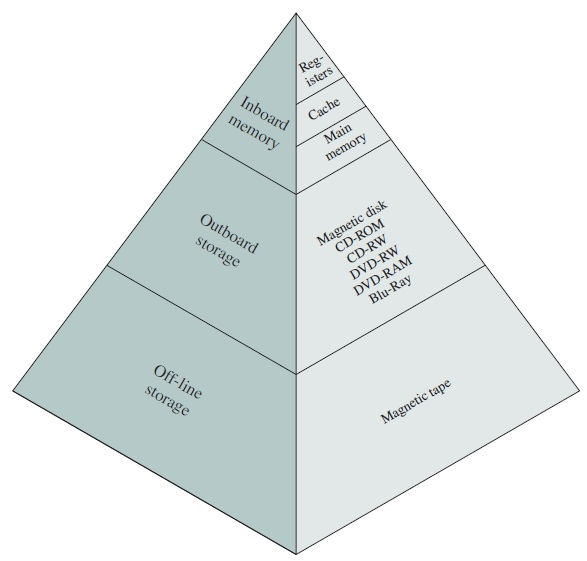
\includegraphics[scale=0.5]{mem_pyramid}
\caption{Hierarchia pamięci\protect\cite{OS_Stallings}}
\label{fig:mem_pyramid}
\end{figure}

\indent Na samym szczycie hierarchii stoją rejestry procesora,
w których zawierają się instrukcje, dane i adresy z pamięci pobierane z pamięci niższego poziomu, wykorzystywane przez \textbf{ALU} oraz jednostkę zapisu i odczytu. Jako bufor do wymiany danych z pamięcią główną, jest wykorzystywana pamięć podręczna procesora - CPU cache(patrz rys. \ref{fig:cache_mem}).
Cache jest obecnie najczęściej podzielony na trzy poziomy - 
L1, L2, L3. Każdy z nich posiada kopię fragmentu pamięci głównej, gdzie największy jest zawarty w L3 cache, a najmniejszy w L1.
Jeśli procesor potrzebuje pobrać dane z adresu w pamięci głównej, którego kopia nie jest w L1, sprawdzany jest cache L2, 
następnie L3. 
\\
\indent Poprzez zastosowanie hierarchicznego modelu pamięci,
zwiększyła się istotność w programowaniu sekwencyjnym jak i współbieżnym, brania pod uwagę budowy pamięci podręcznej.
Cache składa się z linii odpowiadających blokom z pamięci głównej. Jeśli potrzebny adres bloku pamięci głównej
nie występuje w cache'u, musi być pobrany z pamięci głównej,
zapisany w nim oraz przekazany do rejestrów procesora. Dlatego, że cache składa się z kopi kolejnych bloków 
pamięci głównej, przy operacji na tablicach w językach programowania w celu wykorzystania szybkości pamięci podręcznej, należy je przetwarzać wierszami, a nie kolumnami;
zgodnie z kolejności występowania w pamięci.
\cite{Computer_Architecture_Patterson_Hennesy}\cite{OS_Stallings}\cite{Inside_Machine}
%rysunek cache
\begin{figure}[h]
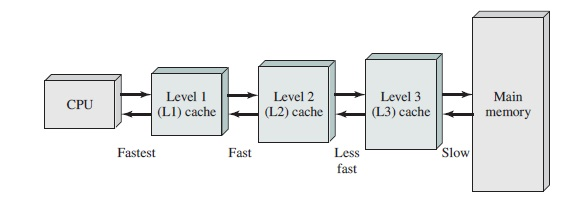
\includegraphics[scale=0.7]{cache}
\caption{Trójpoziomowa organizacja pamięci cache \protect\cite{OS_Stallings}}
\label{fig:cache_mem}
\end{figure}

%\indent%opis pipelinenig - równoległość na poziomie instrukcji
%architektura równoległego przetwarzania danych na CPU
\indent Podstawową metodą zwiększania szybkości wykonywania instrukcji przez procesor jest wykorzystywanie potokowości.
Zgodnie z wcześniej przedstawionym modelem wykonywania instrukcji, każda jest pobierana z pamięci, dekodowana, wykonywana przez procesor, a wynik jest zapisywany do określonego rejestru. Procesory jedno-cyklowe, które wykonują wszystkie powyższe kroki w czasie jednego cyklu zegara są proste w budowie, ale zużywają dużo zasobów sprzętowych ponieważ procesor nie przetwarza więcej niż jednej instrukcji w tym samym czasie.\cite{Inside_Machine}. Stoując mechanizm potokowości(pipelining) cykl przetwarzania instrukcji jest podzielony na odrębne fazy:
\begin{enumerate}
\item Fetch - pobranie instrukcji z pamięci
\item Decode - interpretacja instrukcji
\item Execute - wykonanie instrukcji
\item Write - zapisanie wyniku do rejestru
\end{enumerate}

Gdy pierwsza zostaje zakończona, zaczyna się druga, a pierwsza
zaczyna pobierać następną instrukcję. Analogicznie po dekodowaniu pierwszej instrukcji jest ona wykonywana w 3-ciej fazie, a w tym samym czasie druga instrukcja zaczyna być dekodowana. Zgodnie z tym tokiem postępowania w czasie pierwszego cyklu zegara procesora pobrane zostaną 4 instrukcje, 3 z nich zostaną zinterpretowane, 2 wykonane i wynik jednej będzie zapisany w rejestrze.
\begin{figure}[h]
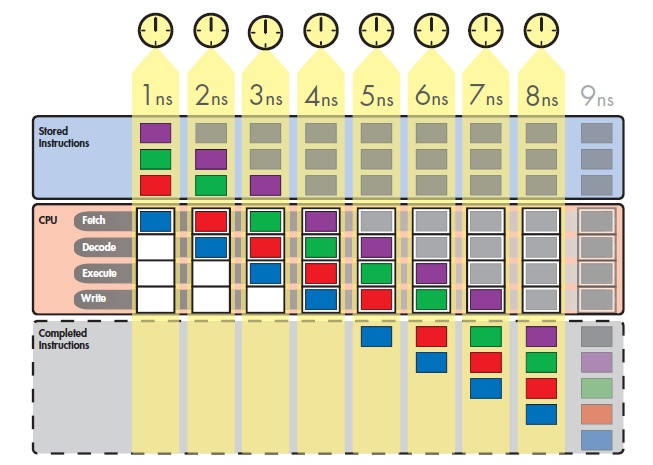
\includegraphics[scale=0.7]{pipeline}
\caption{Przykład 4-fazowego potoku(pipeline) procesora \protect\cite{Inside_Machine}}
\label{fig:pipeline}
\end{figure}
Dla następnego cyklu poprzednio 
nie przetworzone instrukcje zostaną dokończone oraz kolejne 3 zostaną częściowo przetworzone, a pierwsza z nowych instrukcji przejdzie przez wszystkie 4 fazy(patrz rys.\ref{fig:pipeline}).
\cite{Inside_Machine}\cite{Computer_Architecture_Patterson_Hennesy} 
%rysunek pipeline


Wadą zastosowanie potokowości jest zwiększenie złożoności logiki sterowania procesora, ze względu na synchronizację faz przetwarzania instrukcji. Dodatkowo często może dojść do zablokowania jednej z faz potoku, co powoduje opóźnienie w wykonywaniu kolejnych instrukcji. Ponadto szybkość potoku jest zależna od najwolniejszej z faz, która staje się wąskim gardłem całego procesu. Powoduje to sztuczne wydłużenie czasu wykonania pozostałych faz, co bezpośrednio oznacza marnowanie zasobów sprzętowych procesora. Właśnie dlatego, aby koszt zastosowania 
potokowości odpowiadał wzrostowi wydajności procesora, wymagane jest od projektanta CPU zbalansowanie czasu poszczególnych faz potoku. Z tego powodu z czasem zaczęto odchodzić od zwiększania osiągów procesora z wykorzystaniem potokowości. Dalsza współbieżność wykonywania instrukcji programu została oparta na wykorzystaniu technologii wielordzeniowych.\cite{Inside_Machine}\cite{Computer_Architecture_Patterson_Hennesy} 
%model współbieżny na wielu rdzeniach - henessy, net,mimd i te podobne \indent

\indent Innym podejściem do paralelizmu jest sprzętowa implementacja wielowątkowości - \textbf{TLP}(Thread-level parallelism).
\begin{figure}[h]
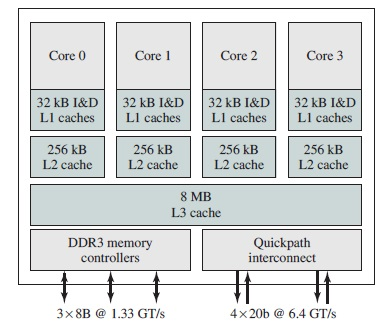
\includegraphics[scale=1]{cpu_i7}
\caption{Intel Core i7, przykład wielordzeniowego procesora wykorzystującego model \textbf{SMT} \protect\cite{OS_Stallings}}
\label{fig:cpu_i7}
\end{figure}
Występują trzy sprzętowe podejścia do realizacji wielowątkowości\cite{Computer_Architecture_Patterson_Hennesy}
(patrz rys.\ref{fig:thread_types}):
\begin{itemize}
\item Fine-grained multithreading(FMT) - przełączanie pomiędzy wątkami występuje 
co każdy cykl procesora. Powoduje to naprzemienne wykonywanie instrukcji, gdzie w przypadku wątków, które czekają na zdarzenie i nie wykonują instrukcji, są one w tym czasie pomijane. Zaletą tego podejścia jest zmniejszenie straty wydajności, spowodowanych przez czekające wątki. Wadą jest zwolnienie wykonywania instrukcji pojedynczego wątku.
\item Coarse-grained mutlithreading(CMP) - alternatywa dla FMT, zmienia obecnie wykonywany wątek, tylko w momencie długotrwałego oczekiwania na kontynuowanie egzekucji(np. brak potrzebnego adresu w cache L2 lub L3). Zaletą tego podejścia jest
zmniejszenie czasu wykonania pojedynczego wątku. 
\item Simultaneus mutlithreading(SMT) - najpopularniejsza implementacja wielowątkowości dla CPU, ulepszona wersja FMT dla
procesorów wielordzeniowych o dynamicznym przydzielaniu.
Pozwala ono na wykonywanie w tym samym cyklu instrukcji z kilku
wątków. Pozwala to na optymalne wykorzystanie możliwości procesora do współbieżnego przetwarzania instrukcji.
\end{itemize}

%rysunek TLP
\begin{figure}[h]
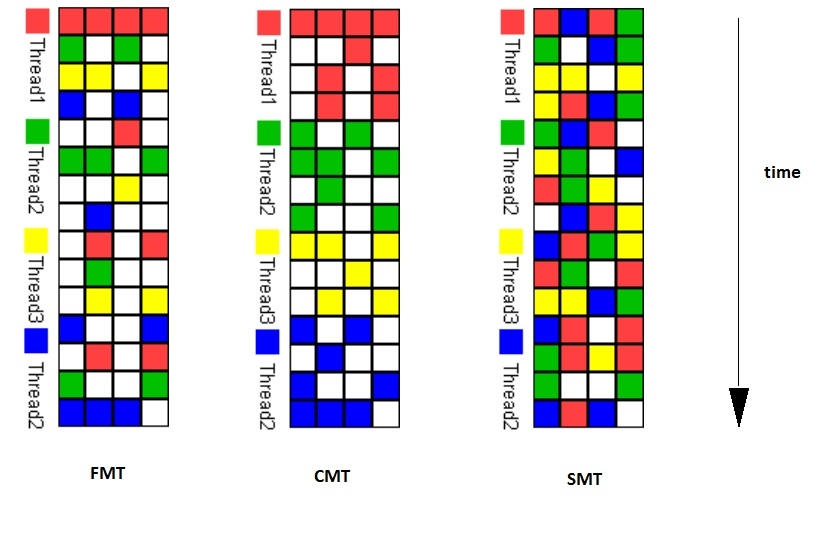
\includegraphics[scale=0.5]{thread_types}
\caption{Rodzaje implementacji \textbf{TLP}}
\label{fig:thread_types}
\end{figure}

\indent Oprócz omówionych wcześniej metod implementacji współbieżności: potokowość - równoległość na poziomie instrukcji
(\textbf{ILP} - instruction-level parallelism), \textbf{TLP},
występuje trzecia kategoria - współbieżność na poziomie danych
(\textbf{DLP} - Data-level parallelism). Polega on na równoczesnym przetwarzaniu wielu strumieni danych.
Wyróżniane są architektury:
\begin{itemize}
\item MIMD - \textit{multiple instruction, multiple data} 
\item SIMD - \textit{single instruction multiple data}
\end{itemize}
\indent Systemy MIMD wspierają jednoczesne wykonywanie wielu instrukcji, operując na wielu strumieniach danych. Składają się z kolekcji niezależnych procesorów lub rdzeni, gdzie każdy posiada własny zestaw rejestrów, ALU i jednostkę kontrolną. Systemy te nie posiadają jednego zegara synchronizującego wszystkie procesory, każdy z nich może pracować asynchronicznie.\cite{openmp_pacheco}\cite{OS_Stallings}.
Występują dwa rodzaje systemów MIMD: współdzielące pamięć(\textit{shared-memory systems} oraz
z oddzielną pamięcią(\textit{distributed-memory systems}).
Pierwsze z nich są kolekcją autonomicznych procesorów połączonych szyną pamięci głównej. Komunikują się ze sobą najczęściej używając współdzielonych obszarów pamięci.
W systemach z oddzielną pamięcią, każdy procesor posiada własną
pamięć prywatną, a komunikacja jest wykonywana poprzez wykorzystywanie specjalnych funkcji sygnalizujących.\cite{OS_Stallings}
\\
\indent Architektura SIMD pozwala wykorzystywać jedną instrukcję do przetwarzania wielu danych. Może być on rozpatrywany
jako jedna jednostka sterująca wyposażona w wiele jednostek ALU.
Posiada najczęstsze zastosowanie w dokonywaniu operacji na tablicach oraz współbieżnego przetwarzania pętli. 
\cite{Computer_Architecture_Patterson_Hennesy}\cite{openmp_pacheco}

%%%%%%%CPU END%%%%%%%%%%%%%}
\clearpage

\section{Wielowątkowość aplikacji dla języka C/C++}
%wstęp równoległość
\indent Najbardziej popularnym podejściem do pisania aplikacji jest sekwencyjne wykonywanie
instrukcji przez procesor - tylko jedna z nich może być wykonywana w tym samym czasie.
Jednak dużą ilość problemów można rozbić na niezależne fragmenty,
które mogą być rozwiązywane równolegle. Obecnie powszechnie stosowane procesory wielordzeniowe dają możliwość rozdzielenia obciążenia obliczeniowego na poszczególne rdzenie oraz dla każdego rdzenia na osobne wątki.\cite{Computer_Architecture_Patterson_Hennesy}\cite{Parallel_computing_article} \\
 %wątek def i opis
 \indent Wątek jest to podproces, który posiada własny stos, zestaw rejestrów, ID, priorytet i wykonuje określony fragment kodu programu. 
 W przeciwieństwie do prawdziwego procesu posiada wspólną pamięć globalną i sterty, dzieloną z innymi wątkami istniejącymi w ramach tego samego procesu. 
 Wątki procesu wykonują się równolegle, dopóki nie potrzebują dostępu do zasobów we wspólnej pamięci.\cite{POSIX_article}\cite{POSIX_tutorial} 
 Wtedy ze względu na problem błędnego odczytu, bądź zapisu wartości w pamięci kiedy inny wątek ją już nadpisał, może spowodować niewłaściwe działanie programu. 
 Fragmenty kodu gdzie może dojść do tego problemu nazywane są sekcjami krytycznymi. Do zabezpieczania sekcji krytycznych programu stosowane są blokady - muteksy(Mutual exclusions) oraz zmienne warunkowe.
 Zastosowanie muteksa powoduje, że w danym momencie tylko jeden wątek może wykonywać kod chroniony przez tą blokadę i dopóki nie opuści chronionej sekcji krytycznej inny wątek nie może zacząć jej wykonywać. 
 Zmienne warunkowe stosowane są do sygnalizowania postępu danego wątku, tak aby inny mógł kontynuować wykonywanie operacji sekcji krytycznej. 
 Stosowane razem z blokadami umożliwiają właściwą synchronizację pracy wątków tego samego procesu.
\cite{POSIX_Butenhof}\cite{C++_Stroustrup} \\
 %watek - wady i zalety 
\indent Używanie wielowątkowości w aplikacjach pozwala na wykorzystanie możliwości sprzętowych procesorów wielordzeniowych do obliczeń równoległych.
Ponadto wielowątkowy model programowania umożliwia wykonywanie przez proces dalszych działań w czasie czasochłonnych obliczeń, bądź czekania na zdarzenie blokujące - takie jak ,np.sygnał z urządzenia peryferyjnego.
Wadą tworzenia dodatkowych wątków w programie jest narzut obliczeniowy
związany z ich synchronizacją(omawiany wcześniej problem wyścigu oraz zjawisko zakleszczenia - wątki czekają na siebie nawzajem żeby móc kontynuować obliczenia) oraz dostępem do wspólnego obszaru pamięci.\cite{POSIX_Butenhof}\cite{C++_Stroustrup} \\
%podsumowanie
\indent W tym rozdziale zostaną omówione różne metody tworzenia aplikacji
wielowątkowych w języku C/C++. Skupiono się na bibliotekach dla tych języków
programowania ze względu na ich popularność w tworzeniu rozwiązań dla systemów wbudowanych, która wynika z wysokiej wydajności kodu i małego zużycia pamięci w porównaniu do języków interpretowanych, np. Java, Python.\cite{C++_Stroustrup}\cite{C_King}

\subsection{Biblioteka POSIX dla systemów Unix}
\indent Dla systemów z rodziny Unix w 1995 ustalony został standard programowania 
wielowątkowego nazywany POSIX threads, w skrócie Pthreads. API Pthreads zostało zdefiniowane jako zestaw typów i procedur w języku C, zawarte w pliku nagłówkowym
\code{<pthread.h>} i bibliotece libpthread.\cite{POSIX_article}
Korzystanie z biblioteki Pthreads do tworzenia wątków generuje mniejszy narzut
niż tworzenie osobnych procesów do równoległego przetwarzania danych.\cite{POSIX_article} 
\\
\indent Wątek w programie jest reprezentowany poprzez zmienną typu \code{pthread\_t}, 
najczęsciej zdefiniowaną jako zmienna statyczna lub jako struktura, która jest zaalokowana na stercie.\cite{POSIX_Butenhof}\cite{POSIX_article}\cite{POSIX_tutorial} 
Do każdego stworzonego wątku przypisana jest funkcja, którą będzie wykonywał.
Funkcja powinna przyjmować jako argument zmienną wskaźnikową \code{void*} i zwracać
wartość tego samego typu. Za tworzenie nowego wątku odpowiedzialna jest funkcja \code{pthread\_create}. Przyjmuje ona adres funkcji oraz argument z jakim ma zostać wywołana.
Wywołanie \code{pthread\_create} oprócz rozpoczęcia nowego wątku zwraca identyfikator
\code{pthread\_t}, który będzie wykorzystywany do odnoszenia się do stworzonego wątku.
Wątek zostaje zakończony jeśli wykona wszystkie instrukcje swojej funkcji lub jeśli wywoła procedurę \code{pthread\_exit}. \cite{POSIX_Butenhof}

\begin{figure}[h]
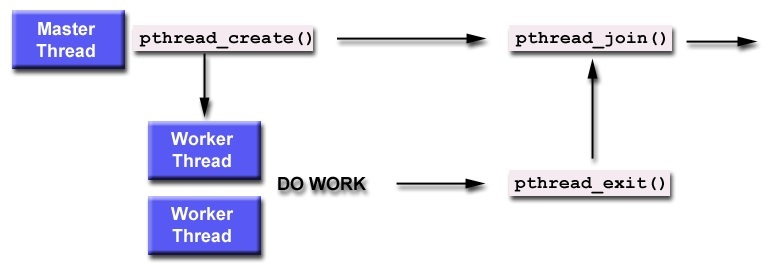
\includegraphics[scale=0.7]{posix_thread_tree}
\caption{Wykorzystanie \code{pthread\_join} do synchronizacji wątków\protect\cite{POSIX_article}}
\label{fig:inspekcja}
\end{figure}

Jedną z podstawowych metod synchronizacji pomiędzy wątkami jest użycie funkcji \code{pthread\_join}, która powoduje zatrzymanie dalszego wykonywania instrukcji dopóki stworzony wątek nie zakończy pracy.
Tylko wątki, które został stworzone z atrybutem \code{joinable}, 
a nie \code{detached}(odłączony) mogą używać tego rodzaju synchronizacji.\cite{POSIX_article}(patrz \ref{lst:basic_thread}). % kontynuować o wątkach
\\
\lstinputlisting[language=C, label={lst:basic_thread}, caption=Przykład tworzenia i uruchamiania wątków]{code_snippets/posix_example_0.c} 

\indent W celu zapewnienia bezpieczeństwa w współdzieleniu zasobów
pomiędzy wątkami podczas wykonywania sekcji krytycznych,
najpopularniejsze jest wykluczenie jednoczesnego czytanie bądź zapisu
wartości w dzielonej pamięci. Używane do tego są zmienne wzajemnego
wykluczenia - w skrócie muteks(mutual exclusion). Muteks jest szczególnym przypadkiem semaforu Dijkstry - semaforem binarnym 
o zbiorze wartości {0, 1}.\cite{POSIX_Butenhof}\cite{POSIX_tutorial}\cite{POSIX_article} 
W bibliotece POSIX threads muteks jest reprezentowany jako zmienna typu \code{pthread\_mutex\_t}. W celu posiadania globalnego
zasięgu deklarowana jest jako zmienna \code{static} lub \code{extern}.
\cite{POSIX_Butenhof}\cite{C_King}(patrz\ref{lst:mutex_thread})
W celu deklaracji muteksa wykorzystywane jest makro \code{PTHREAD\_MUTEX\_INITIALIZER}(patrz . Jeśli muteks jest używany jako
element dynamicznie alokowanej struktury, musi zostać zainicjalizowany 
wywołaniem funkcji \code{pthread\_mutex\_init}. Ponadto musi być w ten
sposób inicjalizowany, jeśli nie ma posiadać domyślnych atrybutów.
Niezbędne jest po zakończeniu używania muteksa, zwolnienie zaalokowanej pamięci, poprzez wykorzystanie funkcji \code{pthread\_mutex\_destroy}.\cite{POSIX_Butenhof} 
\\
\lstinputlisting[language=C, label={lst:mutex_thread}, caption=Przykład wykorzystanie muteksa do synchronizacji
aplikacji wielowątkowej]{code_snippets/posix_example_1.c}

\indent Pthreads do komunikacji pomiędzy wątkami wykorzystuje zmienne
warunkowe(condition variables), które mają informować o stanie 
współdzielonych zasobów. Używane razem z muteksami, w atomiczny 
sposób zwalniają blokadę sekcji krytycznej, dopóki inny wątek nie
zasygnalizuje kontynuacji używając funkcji \code{pthread\_cond\_signal}. Dzięki temu inny wątek może kontynuować pracę 
zanim zostanie wykonana chroniona sekcja krytyczna.

\indent Dzięki przedstawionym metodom sygnalizacji stanu oraz 
blokadom, możliwe jest zaprojektowanie pożądanego podziału obciążenia
obliczeniowego. Biblioteka POSIX, choć wiekowa dalej jest stosowana
dzięki małemu narzutowi(napisana w języku C), obszernej dokumentacji 
oraz dużej ilości starego kodu, który dalej jest stosowany w nowych
rozwiązaniach systemów wbudowanych i czasu rzeczywistego.\cite{POSIX_tutorial}

%%%%%%%%%%%%%%%%%%%%%%%%%%%%%%%%%%%%%%%%%%%%%%%%%%%%%%%%%%%%%%%%%%%
\subsection{OpenMP - wieloplatformowe API}
%żródła do tego rozdziału
%\cite{openmp_pacheco}
%\cite{openmp_spec}
%\cite{openmp_guide}
%\cite{openmp_slides}
%--------------------------
\indent Podobnie jak Pthreads, OpenMP jest biblioteką wykorzystującą
model współdzielenia pamięci do programowania równoległego. Zawiera wsparcie dla języków C, C++ oraz Fortran.
OpenMP wymaga sprecyzowania przez użytkownika odpowiednich akcji, które ma wykonać kompilator, aby program wykonywał się równolegle.
\cite{openmp_pacheco}\cite{openmp_spec}
OpenMP został stworzony przez grupę naukowców i programistów, którzy
uważali, że używanie API Pthreads jest skomplikowane dla dużych
aplikacji. Zdecydowali się stworzyć standard wyższego poziomu, który
w przeciwieństwie do biblioteki Pthreads wymagającej od programisty zdefiniowania funkcji wykonawczej dla każdego wątku, pozwala 
na określenie dowolnego fragmentu programu, który ma być wykonany 
równolegle. Wykorzystuje do tego dyrektywy preprocesora znane jako
\code{\#pragma}.Używane są do zdefiniowania zachowań kompilatora,
które nie są zawarte w podstawowej specyfikacji języka C.
Jeśli użyty kompilator nie wspiera dyrektyw \code{\#pragma}, program
i tak ma możliwość właściwego działania; wtedy jego fragmenty mające wykonać
się równolegle zostaną obsłużone przez jeden wątek.
\cite{openmp_pacheco}\cite{C_King}\cite{openmp_spec}\cite{openmp_guide}
Oprócz zestawu dyrektyw preprocesora, OpenMP składa się z biblioteki
funkcji i makr, które wymagają dodania pliku nagłówkowego \code{<omp.h>}
z ich definicjami i prototypami.
\\
\indent Podstawową dyrektywą OpenMP jest dyrektywa \code{\#pragma omp parallel},
za pomocą której określany jest blok kodu mający być wykonany wielowątkowo.
Jeśli programista nie sprecyzuje przez ile wątków
ma być przetworzony podany fragment programu, zostanie on określony przez system
wykonawczy(zazwyczaj po jednym wątku na rdzeń).\cite{openmp_pacheco}\cite{openmp_guide}(patrz \ref{lst:openmp_0})
\\
\lstinputlisting[language=C, label={lst:openmp_0}, caption= Prosta aplikacja wykorzystująca dyrektywę \code{\#pragma omp parallel} 
\protect\cite{openmp_pacheco}]{code_snippets/openmp_example_0.c}

Powyższy prosty przykład ilustruje wykorzystanie OpenMP do równoległego
uruchomienia \code{thread\_count} wątków, gdzie każdy z nich wykona
funkcję \code{mp\_test}.Dodatkowo użyta klauzula \code{num\_threads}
modyfikuję dyrektywę tak aby stworzyła tyle wątków ile zostało 
podane w liście argumentów przy uruchomieniu programu(wskaźnik na tablicę \code{argv}). Jeśli jeden z wątków wcześniej skończy pracę od innych,
czeka aż reszta zakończ wykonywanie funkcji \code{mp\_test}.
Każdy ze stworzonych wątków otrzymuje swoje id, stopień oraz parametr
określający liczbę innych wątków w ramach tego samego bloku.
Korzystając z funkcji \code{omp\_get\_thread\_num} i \code{omp\_num\_threads}
(nagłówek \code{<omp.h>}) otrzymywane jest id i liczba współpracujących wątków.
Współdzielonym zasobem pomiędzy wątkami jest strumień wyjściowy \code{stdout}.
\cite{openmp_pacheco}\cite{openmp_slides}
\\
\indent Kolekcja wątków wykonujących blok kodu nazywana jest zespołem. Wątek,
który przetwarzał instrukcje przed dyrektywą \code{\#pragma omp parallel} 
jest zarządcą(\textbf{master}), a dodatkowe wątki są jego podwładnymi(\textbf{slave}). Kiedy wszystkie zakończą swoją pracę łączą się z
wątkiem twórcą, który wtedy kontynuuje wykonywanie dalszych instrukcji(patrz rys. \ref{fig:openmp_tree}).\cite{openmp_blaise}\cite{openmp_spec}

\begin{figure}[h]
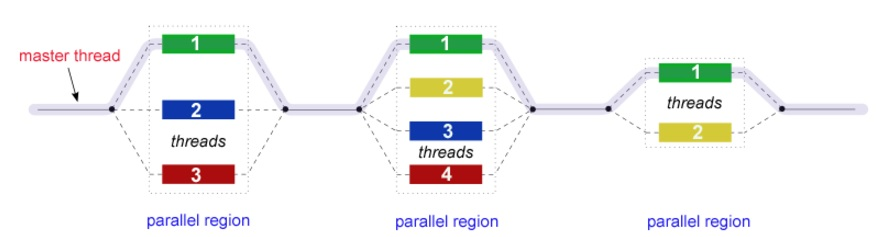
\includegraphics[scale=0.7]{openmp_tree}
\caption{Model tworzenia wątków w OpenMP\protect\cite{openmp_blaise}}
\label{fig:openmp_tree}
\end{figure}

\indent Podobnie jak dla Pthreads OpenMP uwzględnia ochronę sekcji krytycznej 
oraz metody synchronizacji wątków. Do przeciwdziałania wyścigom i zakleszczeniom(deadlocks) pomiędzy wątkami wykorzystywane są:\cite{openmp_spec}\cite{openmp_guide}
\begin{itemize}
\item Dyrektywa \code{critical} - tylko jeden wątek może w tym samym czasie wykonywać blok strukturalny. Możliwe jest istnienie wielu sekcji \code{critical}, gdzie ich nazwy 
są używane jako globalne identyfikatory. Różne regiony \code{critical} o tej samej
nazwie są traktowane jako jedna sekcja.\cite{openmp_pacheco}\cite{openmp_blaise} 
\begin{verbatim}
#pragma omp critical [ nazwa ]
{
   blok strukturalny
}
\end{verbatim}

\item Dyrektywa \code{atomic} - wykorzystuje specjalne instrukcje sprzętowe, dzięki
czemu możliwa jest dużo szybsza realizacja sekcji krytycznej. Atomowe operacje to
takie które wykonywane są zawsze całkowicie, bez interwencji innego wątku.
Najczęściej sekcje \code{atomic} używane są do prostych operacji na licznikach
zmienianych przez kilka wątków równolegle.\cite{openmp_guide}\cite{openmp_spec}
\\
Operacje zmiany zmiennej:
\begin{verbatim}
#pragma omp atomic [ nazwa ]
{
   ++x; --x; x++; x--;
   x += expr;  x -= expr;  x *= expr;   x /= expr;  x &= expr;
   x = x+expr; x = x-expr; x = x*expr;  x = x/expr; x = x&expr;
   x = expr+x; x = expr-x; x = expr*x;  x = expr/x; x = expr&x;
   x |= expr;  x ^= expr;  x <<= expr;  x >>= expr;
   x = x|expr; x = x^expr; x = x<<expr; x = x>>expr;
   x = expr|x; x = expr^x; x = expr<<x; x = expr>>x;
}
\end{verbatim}

Operacje czytania i nadpisania zmiennej:
\begin{verbatim}
#pragma omp atomic [ nazwa ]
{
   var = x++;
   var = x; 
   x++;
   x = expr;
}
\end{verbatim}
\item Blokada \code{omp\_lock\_t} z pliku nagłówkowego \code{<omp.h>} - ogranicza dostęp
do funkcji krytycznej. Posiada pięć funkcji do manipulacji blokadą \cite{openmp_guide}\cite{openmp_blaise}:
	\begin{itemize}
	\item \code{omp\_init\_lock} - inicjalizuje blokadę. Po tym wywołaniu nie jest jeszcze ustawiona.
	\item \code{omp\_destroy\_lock} - usuwa blokadę, nie może być wcześniej ustawiona.
	\item \code{omp\_set\_lock} - próbuje ustawić blokadę. Jeśli inny wątek już wywołał tą
	funkcję, czeka aż blokada będzie znowu dostępna, wtedy zostaje ona ustawiona.
	\item \code{omp\_unset\_lock} - zwalnia blokadę, powinna być użyta tylko przez wątek,
	który ją ustawił. W innym wypadku zachowanie programu będzie niezdefiniowane.
	\item \code{omp\_test\_lock} - próbuje ustawić blokadę. Jeżeli jest już ustawiona 
	przez inny wątek, zwraca 0. Jeśli nie, blokuje sekcję krytyczną i zwraca 1.
	\end{itemize}
\end{itemize}

\indent OpenMP umożliwia automatyczne podzielenie pomiędzy wątki iteracji pętli \code{for}. 
Używana jest do tego dyrektywa \code{\#pragma omp for}, która rozdziela na sekcję rozpatrywaną pętlę, pomiędzy wszystkie stworzone wątki w ramach tego bloku strukturalnego.
\cite{openmp_guide}\cite{openmp_pacheco}
\begin{verbatim}
#pragma omp parallel num_threads(n)
{
   #pragma omp for
   {
      for(int i = 0; i < 10; i++)
      {
         cout << i << endl;
      }  
   }
}
\end{verbatim}

\indent Zasięg zmiennych jest zależny od tego czy są one zdefiniowane przed blokiem strukturalnym, czy wewnątrz niego. Zmienne zdefiniowane przed dyrektywą \code{parallel}
albo \code{for}, są widoczne dla każdego wątku. Te których deklaracje są wewnątrz
konstrukcji OpenMP, są prywatne dla każdego stworzonego wątku w tym bloku.
Będą one zawierać indywidualne kopie tej zmiennej we własnej pamięci stosu.
\cite{openmp_pacheco}\cite{openmp_spec}
\\
\indent Podsumowując, OpenMP jest biblioteką wyższego poziomu, na którą składa się
zestaw dyrektyw preprocesora, makr i funkcji umożliwiających tworzenie aplikacji
wielowątkowych. Jest dobrą alternatywą dla biblioteki Pthreads, ponieważ podobnie jak
ona jest napisana dla języka C i dodatkowo umożliwia korzystanie z nowszych funkcjonalności
języka C++. Upraszcza synchronizację i tworzenie nowych wątków oraz umożliwia bez zmiany
kodu, wykonanie instrukcji programu sekwencyjnie dla kompilatorów niewspierających dyrektyw \code{\#pragma}. W przeciwieństwie do Pthreads nie wymaga określenia konkretnej funkcji,
którą ma wykonywać dany wątek, tylko automatycznie rozdziela wykonywanie instrukcji bloku
strukturalnego(fragment kodu objęty dyrektywą code{\#pragma}) przez ustawioną liczbę stworzonych wątków. Umożliwia inkrementalne zwiększanie
równoległości programu poprzez dodawanie kolejnych dyrektyw i elementów biblioteki zdefiniowanych w nagłówku \code{<omp.h>}

\subsection{Wielowątkowość w standardzie C++11}
\indent Nowy standard języka C++ - C++11, istotnie zmienił podejście do pisania programów w porównaniu do starszej wersji C++98. Zamiarem komisji standaryzacyjnej było stworzenie bardziej czytelnego, prostszego w pisaniu oraz bardziej zoptymalizowanego języka.
Wśród wielu nowości, takich jak inteligentne wskaźniki, operator przenoszenia, konstruktor przenoszący, wyrażenia lambda, dedukcja typu auto; jednym z najistotniejszych było wprowadzenie współbieżności do biblioteki standardowej.
Rezultatem tego jest umożliwienie tworzenie wieloplatformowych aplikacji 
wielowątkowych bez potrzeby używania dodatkowych bibliotek, takich jak Pthreads,
Windows threads, OpenMP.\cite{C++_Meyers}\cite{C++_Stroustrup}
\\
\indent Biblioteka standardowa C++11 umożliwia dwie metody wykonywania
zadań asynchronicznie\cite{C++_Meyers}\cite{C++11_iso}:
\begin{itemize}
\item Z wykorzystaniem obiektów typu \code{std::thread}
\item używając podejścia zadaniowego dla obiektów \code{std::future}
\end{itemize}
\indent Podobnie jak dla Pthreads, wielowątkowość implementowana z pomocą
\code{std::thread}, zakłada tworzenie nowych wątków z unikalnymi id, 
pamięcią stosu, funkcją wykonawczą oraz listą argumentów do tej funkcji.
Każdy stworzony wątek może być typu \code{joinable}, albo \code{detached}.
\code{Joinable} oznacza, że wątek powinien zakończyć działanie przed
wywołaniem swojego destruktora. Niezbędne jest zastosowanie do tego 
przez wątek twórcy metody \code{join()}, która zapewnia, że stworzony
wątek wykona swoje zadanie zanim zostanie zniszczony. Jeśli pożądane
jest pozwolenie wątkowi na pracę po wywołaniu jego destruktora, 
używana jest metoda \code{detach()}.\cite{C++11_iso}\cite{C++_Stroustrup}
\\
\indent Analogicznie do POSIX threads, do synchronizacji wykorzystywane są blokady w postaci muteksów  \code{std::mutex} oraz zmienne warunkowe do generacji zdarzeń 
\code{std::condition\_variable}. W celu usunięcia konieczności ręcznego
ustawiania i odblokowywania mutexa(\code{mutex.lock()}, \code{mutex.unlock()}),
wykorzystywany jest obiekt \code{std::lock\_guard}, który po inicjalizacji
muteksem jako argument, ustawia blokadę i zapewnia jej usunięcie po wyjściu
z zasięgu swojej deklaracji(patrz listing \ref{lst:cpp_thread}).\cite{C++11_iso}\cite{C++11_tutorial}
\\
\lstinputlisting[language=C++, label={lst:cpp_thread}, caption= Podstawowe funkcjonalności \code{std::thread} \protect\cite{C++_ref}]{code_snippets/cpp_example_0.cpp}
\clearpage
\indent Innym podejściem do współbieżności, które zostało zawarte w nowym standardzie,
jest współbieżność zadaniowa. Daje ona możliwość wykonania zadania - funkcji i  następnie zwraca
jeden wynik. Wsparcie do tego modelu jest zaimplementowane w postaci\cite{C++_ref}\cite{C++_Meyers}
(patrz listing \ref{lst:cpp_future}) :
\begin{itemize}
\item Typów \code{std::future} i \code{std::promise}. Pierwszy z nich zawierać będzie wynik 
zadania. Po zakończeniu zadania drugi jest używany do odczytywania tej wartości. 
\item \code{std::packaged\_task<T>} - pakuje obiekt typu T do wykonania jako zadanie. Jego konstruktor
przyjmuje przy inicjalizacji funkcję, która ma zostać wykonana asynchronicznie. Wynik otrzymywany ze
stworzonego na bazie funkcji \code{get\_future()}, obiektu \code{std::future} używając metody \code{get()}.
\item funkcji \code{std::async()} - odpowiada za asynchroniczne uruchomienie funkcji podanej w liście argumentów funkcji. 
Zwraca obiekt typu \code{std::future}, z którego możemy otrzymać wynik używając metody \code{get}
\end{itemize}

\lstinputlisting[language=C++, label={lst:cpp_future}, caption= Przykład zastosowania
 \code{std::future} i \code{std::async()} \protect\cite{C++_ref}]{code_snippets/cpp_example_1.cpp}
 
Zaletą tego podejścia jest jego prostota. Kiedy nie potrzebujemy skomplikowanej synchronizacji pomiędzy wątkami,
tylko wiemy, że każdy z nich ma wykonać równolegle niezależne zadanie, jest to wygodniejsza
 metoda pisania aplikacji wielowątkowych. 
\cite{C++_Meyers}\cite{C++_Stroustrup}

\indent Reasumując, standard C++11 umożliwił programistom tworzenie 
aplikacji wielowątkowych z użyciem wyłącznie biblioteki standardowej.
Wątki w C++11 wspierają nowe elementy standardu takie jak, 
funkcje lambda ,referencje do \code{rvalue}, \code{std::bind} oraz wiele innych. Jest to dodatkowe ułatwienie pisania programów, gdzie nie musimy
przejmować się kompatybilnością wykorzystywanej biblioteki. Wystarczające 
jest używanie nowego kompilatora wspierającego C++11. 


%%%%%%%%%%%%%%%%%%%%%%%%%%%%%%%%%%%%%%%%%%%%%%%%%%%%%%koniec rozdziału

\clearpage


\section{Programowanie równoległe z wykorzystaniem GPU}

\subsection{Architektura GPU}

\indent GPU(\textit{graphics processing unit}) jest to  
procesor wyspecjalizowany pod kątem wykonywania elementów potoku
graficznego oraz operacji zmiennoprzecinkowych. Obecne procesor graficzne
są procesorami wielordzeniowymi zaprojektowanymi specjalnie do wykonywania 
równoległych obliczeń. Charakteryzującą metodą osiągania współbieżności jest stosowanie architektury \textbf{SIMD} do wykonywania jednej instrukcji dla wielu elementów danych. Dzięki temu możliwe jest dzielenie wykonywania obliczeń poprzez liczne jednostki arytmetyczno-logiczne dla każdego z rdzenii GPU.(patrz rys.\ref{fig:simd_core})\cite{OpenCL_Gaster}\cite{Computer_Architecture_Patterson_Hennesy}
Oprócz wielu ALU pojedynczy rdzeń posiada pamięć lokalną
oraz pamięć dla stałych. Nie wykorzystywana jest hierarchia pamięci jak dla CPU, gdzie aby przyspieszyć 
czytanie danych z pamięci głównej stosowane są 3 poziomy pamięci podręcznej cache. GPU posiada dużo szybszą pamięć globalną, wspólną dla wszystkich rdzeni.

%core simd
\begin{figure}[h]
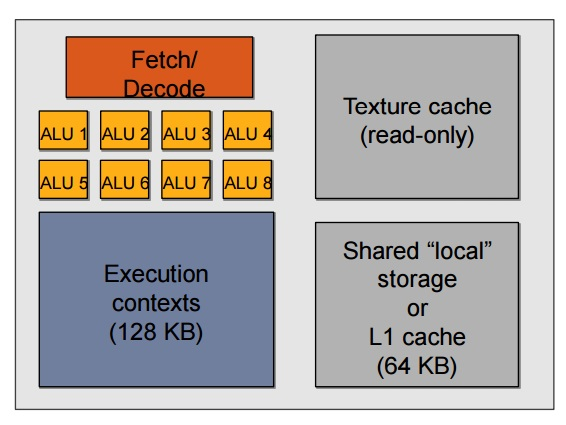
\includegraphics[scale=0.6]{simd_core}
\caption{Schemat rdzenia procesora wykorzystującego architekturę SIMD \protect\cite{Intro_GPU}}
\label{fig:simd_core}
\end{figure}

\indent Stosowanie GPU daje najlepsze rezultaty dla problemów umożliwiającym równoległe przetwarzanie, z dużą ilości operacji arytmetycznych w porównaniu do operacji wymagających dostępu do pamięci.
Dlatego procesory graficzne są najczęściej używane do przetwarzania obrazów, grafiki komputerowej oraz 
czasochłonnych i skomplikowanych arytmetycznie algorytmów.\cite{GPU_Owens}\cite{OpenCL_Gaster}
%cpu vs gpu
\begin{figure}[h]
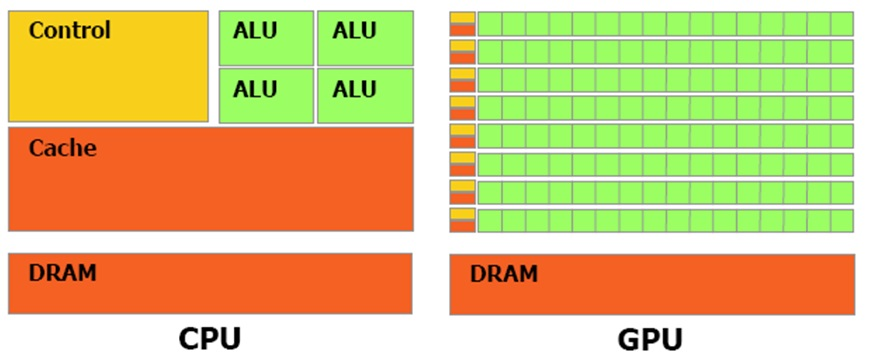
\includegraphics[scale=0.6]{gpu_cpu}
\caption{Porównanie budowy CPU względem GPU\protect\cite{OS_Stallings}}
\label{fig:gpu_cpu}
\end{figure}
%%%%%%%%%%%%%%%%%%%%%%%%%%%%%%%%%%%%%%%%%%%%%%
\subsection{Biblioteka OpenCL}

\indent Bibilioteka OpenCL została stworzona do ułatwienia tworzenia programów dla systemów heterogenicznych. Wykorzystuje trend stosowania rozwiązań wielordzeniowych  w architekturze nowoczesnych procesorów. OpenCL wspiera tworzenie aplikacji dla wielordzeniowych mikroprocesorów , kart graficznych, układów FPGA i DSP.\cite{OpenCL_Gaster}
OpenCL jest to API w języku C z dodatkowymi powiązaniami w językach C++, .NET, Java i Python. Kod przeznaczony dla docelowego urządzenia(CPU lub GPU) jest napisany w języku OpenCL C. Jest to ograniczona wersja języka C w standardzie C99.

\indent Specyfikacja OpenCL jest podzielona na cztery modele\cite{OpenCL_Gaster}\cite{OpenCL_spec}\cite{OpenCL_Banger}:
\begin{enumerate}
\item Model platformy(\textit{Platform model}):
jeden procesor(\textit{Host}) zarządza pracą pozostałych urządzeń(\textit{Device}) wykonujących programy napisane w OpenCL C, zwane kernelami(\textit{kernels}).
Urządzenie jest podzielone na wiele jednostek wykonawczych(\textit{compute units}), gdzie każde z nich składa się z wielu elementów przetwarzania(\textit{processing elements}). Są one odpowiedzialne za przeprowadzanie wszystkich obliczeń.
\item Model wykonawczy(\textit{Execution model}): określa konfigurację środowiska hosta oraz ustawień kerneli.
\item Model pamięci(\textit{Memory model}): definiuje hierarchię pamięci używaną przez kernele
\item Model programistczny(\textit{programming model}): 
określa dwa rodzaje współbieżności - zadaniową(\textbf{TLP}) i danych(\textbf{DLP}), który jest uważany za preferowany dla aplikacji OpenCL.

\end{enumerate}

\begin{figure}[h]
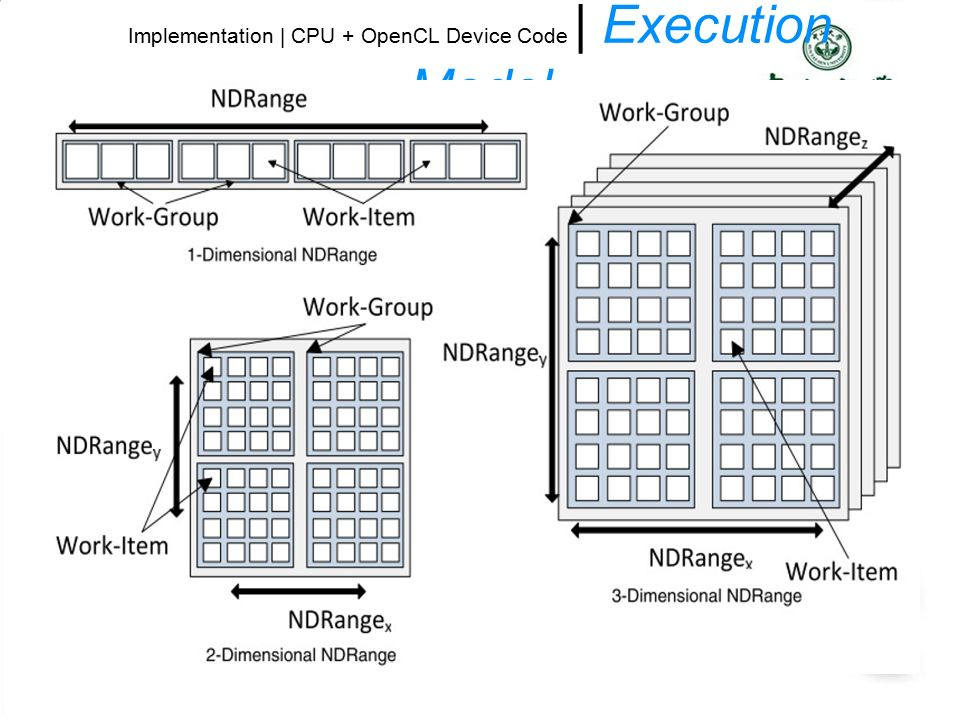
\includegraphics[scale=0.6]{work_group}
\caption{Przestrzeń indeksowa OpenCL \protect\cite{OpenCL_spec}}
\label{fig:work_group}
\end{figure}

%opis co to kernel, work group work item
\indent Wykonywanie programu opartego o OpenCL składa się z dwóch części - instrukcji hosta oraz kerneli przetwarzanych urządzenia OpenCL. Host definiuje abstrakcyjny kontener zwany kontekstem(\textit{context}),
który służy do interakcji z urządzeniami OpenCL, zarządzania pamięcią i nadzorowaniem programów i kerneli
wykonywanych przez każde urządzenie. 
Po zdefiniowaniu i inicjalizacji kernela przez hosta
tworzona jest N wymiarowa przestrzeń indeksowa. Instancja
programu jest wykonywana dla każdego z elementów przestrzeni, które nazywane są elementami roboczymi(\textit{work-item}). Są one zorganizowane
w grupy robocze(\textit{work-groups}), gdzie każda grupa posiada unikalne ID. Każdy element roboczy posiada ID globalne względem całej przestrzeni indeksowej(zwanej też \textit{NDRange}) oraz lokalne w ramach swojej grupy roboczej. Przestrzeń indeksowa może mieć maksymalnie trzy wymiary(patrz rys.\ref{fig:work_group}).\cite{OpenCL_Gaster}\cite{OpenCL_spec}\cite{OpenCL_Banger}

%opis jak wygląda hierarchia pamięci
\indent W ramach kernela OpenCL, dla każdego elementu
roboczego dostępne są(patrz rys.\ref{fig:opencl_memory})
\begin{itemize}
\item pamięć globalna(\textit{global memory}): wspólna dla wszystkich elementów przestrzeni indeksowej.
\item pamięć stała(\textit{constant memory}): po inicjalizacji przez hosta nie zmienia się w czasie wykonywania programu. Możliwe jest tylko odczytywanie danych.
\item pamięć lokalna(\textit{local memory}): indywidualna dla każdej grupy roboczej.
\item pamięć prywatna(\textit{private memory}): osobna dla każdego elementu roboczego, nie jest widoczna dla pozostałych
\end{itemize}

\begin{figure}[h]
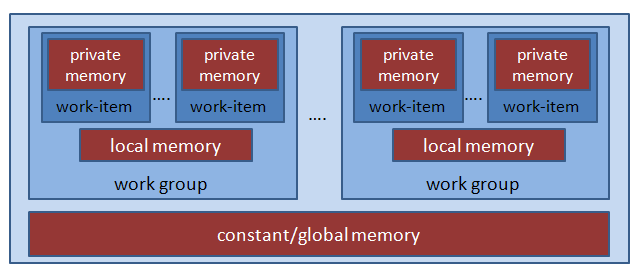
\includegraphics[scale=0.6]{opencl_memory}
\caption{Model pamięci urządzenia OpenCL \protect\cite{OpenCL_spec}}
\label{fig:opencl_memory}
\end{figure}

%flow
\indent Typowa aplikacja wykorzystująca bibliotekę OpenCL
składa się z(patrz listing \ref{lst:opencl_basic}):
\begin{enumerate}
\item Pobrania informacji na temat platformy(wersja API, profil)
\item Określenia listy dostępnych urządzeń i wybrania pożądanych
\item Stworzenia kontekstu dla urządzenia do zarządzania pamięcią, kolejkami rozkazów oraz kernelami
\item Inicjalizacji kolejki rozkazów(\textit{commad queue})
\item Stworzenia buforów pamięci wykorzystywanych do 
wymiany danych pomiędzy hostem a urządzeniem OpenCL.
\item Zbudowanie programu w OpenCL C i stworzenie kernela 
\item Powiązanie buforów z argumentami kernela
\item Wykonanie kernela na urządzeniu
\item Odczytanie przez hosta wyników z buforów pamięci
\item Zakończenie programu urządzenia i zwolnienie pamięci dla wszystkich  obiektów i buforów.
\end{enumerate}

\lstinputlisting[language=C, label={lst:opencl_basic}, caption=Przykład programu wykorzystującego OpenCL\protect\cite{OpenCL_Banger}]{code_snippets/opencl_example_0.c} 
\end{document}
